\documentclass[10pt]{exam}
\firstpageheader{Math 4050}{Worksheet \#1}{Name: Sunny Lee}
\usepackage{amsfonts}
\usepackage{amsmath}
\usepackage{amssymb, graphicx, enumerate, mathrsfs}

\begin{document}

\begin{enumerate}
    \item Plotting the points: \\ 
    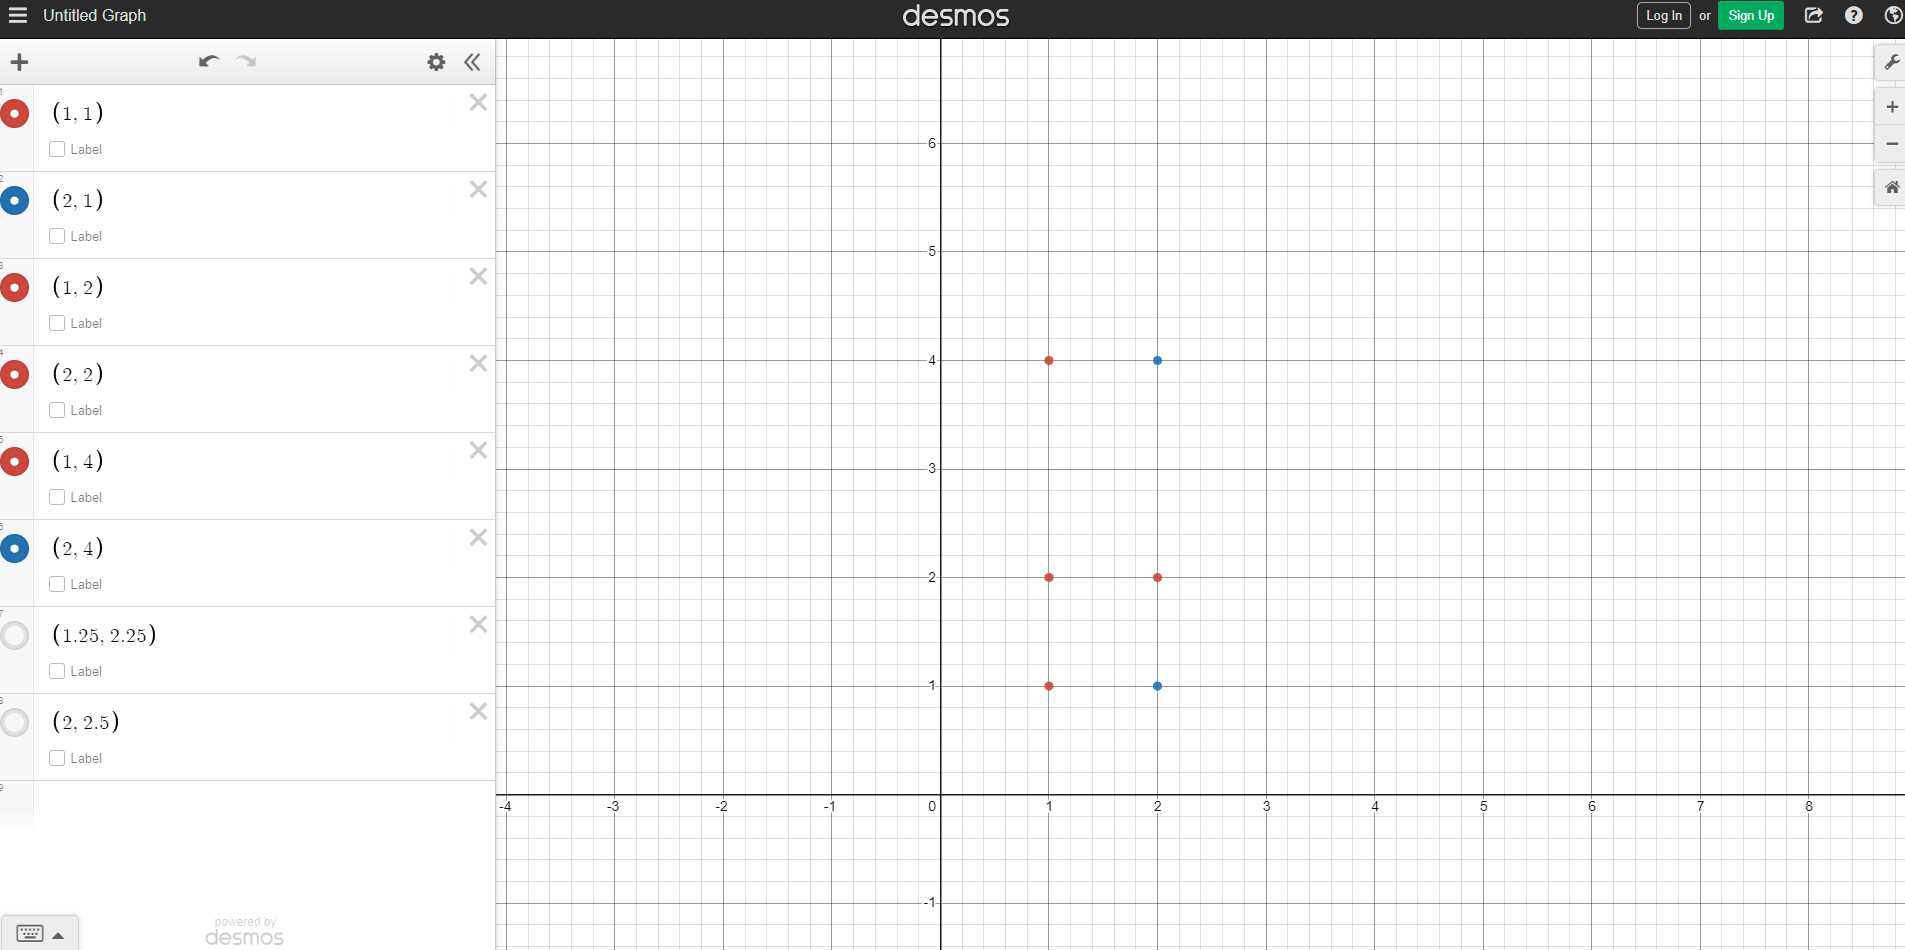
\includegraphics[scale = .3]{1.png}
    
    \item 
    \begin{enumerate}
        \item Finding the centroids: \\ 
        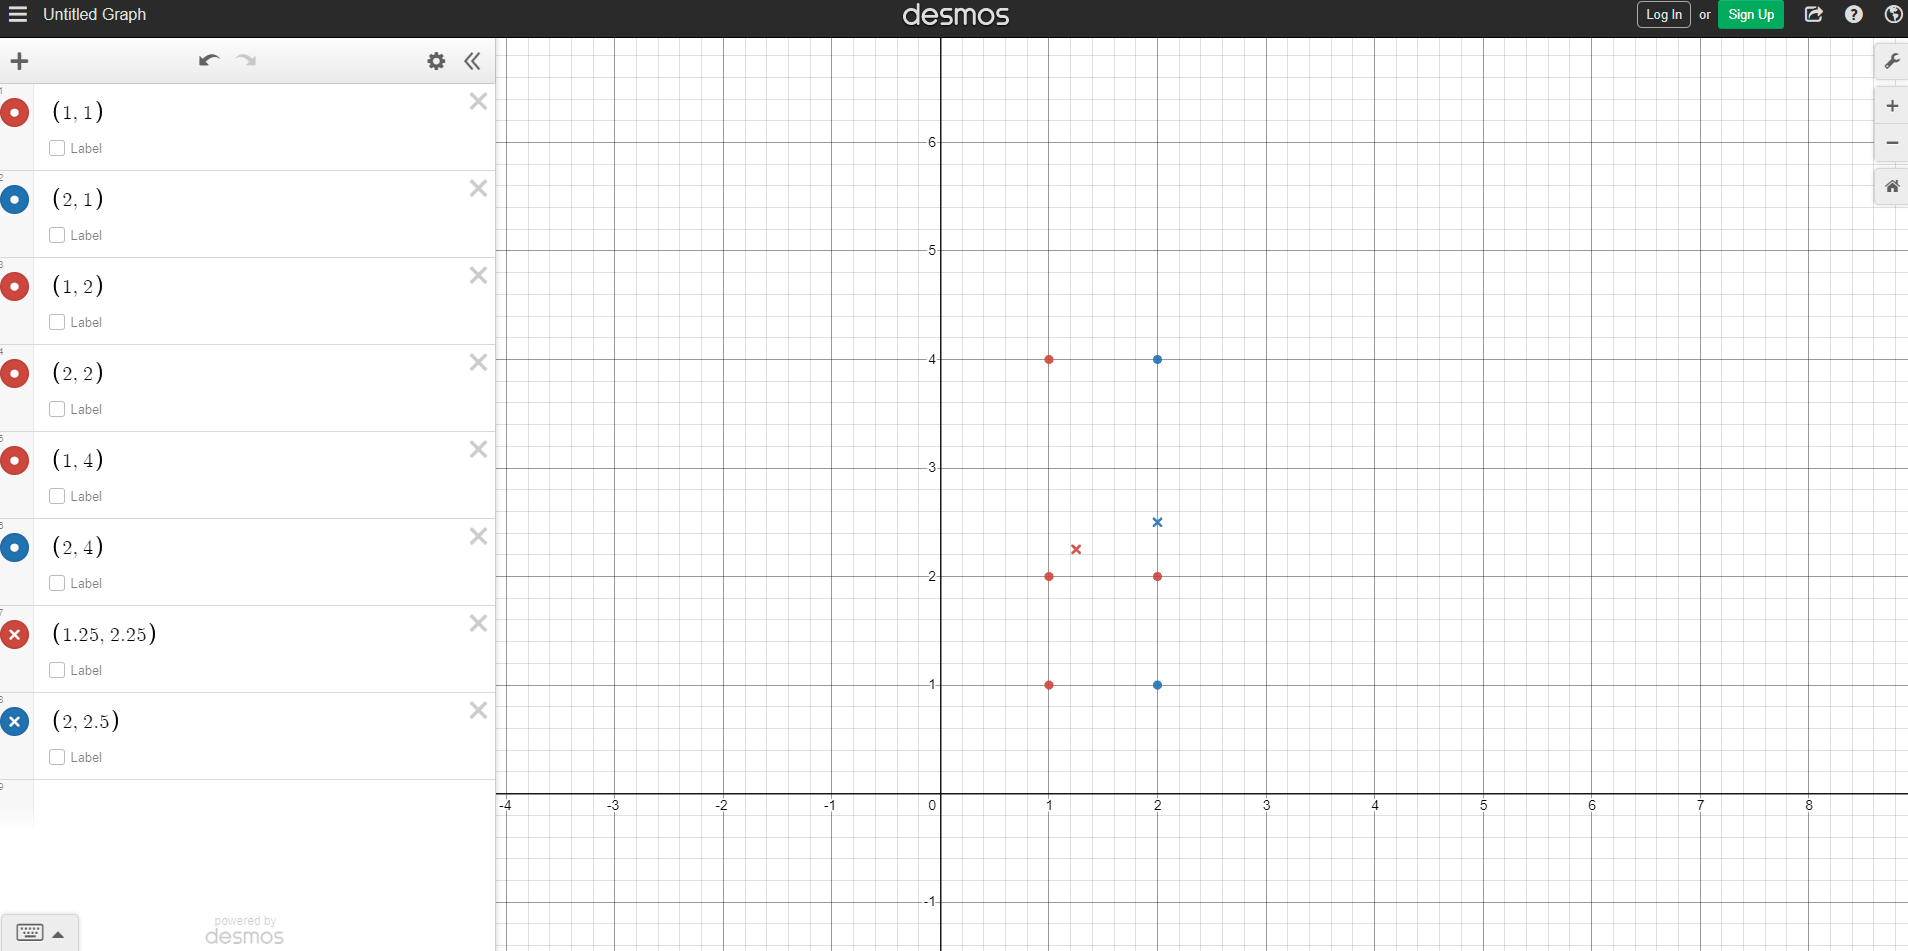
\includegraphics[scale = .3]{2a.png}
        \item Re-assigning the points: \\ 
        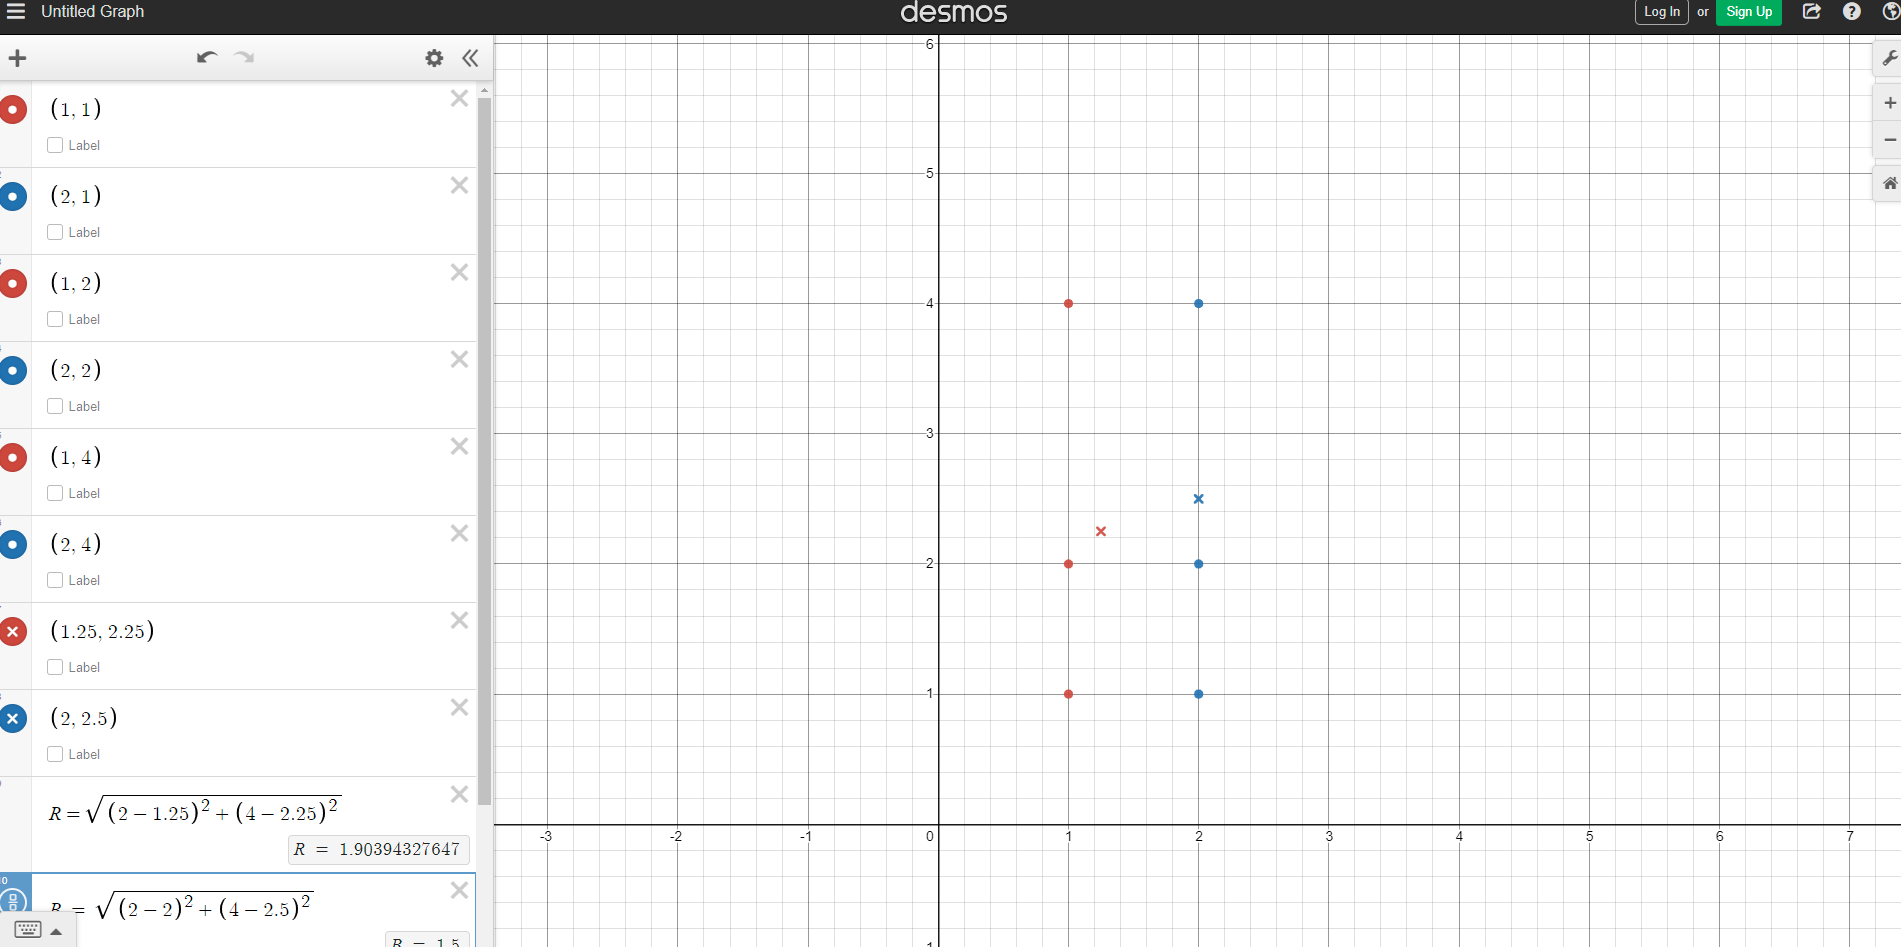
\includegraphics[scale = .3]{2b.png}
        \item In the next iteration: \\ 
        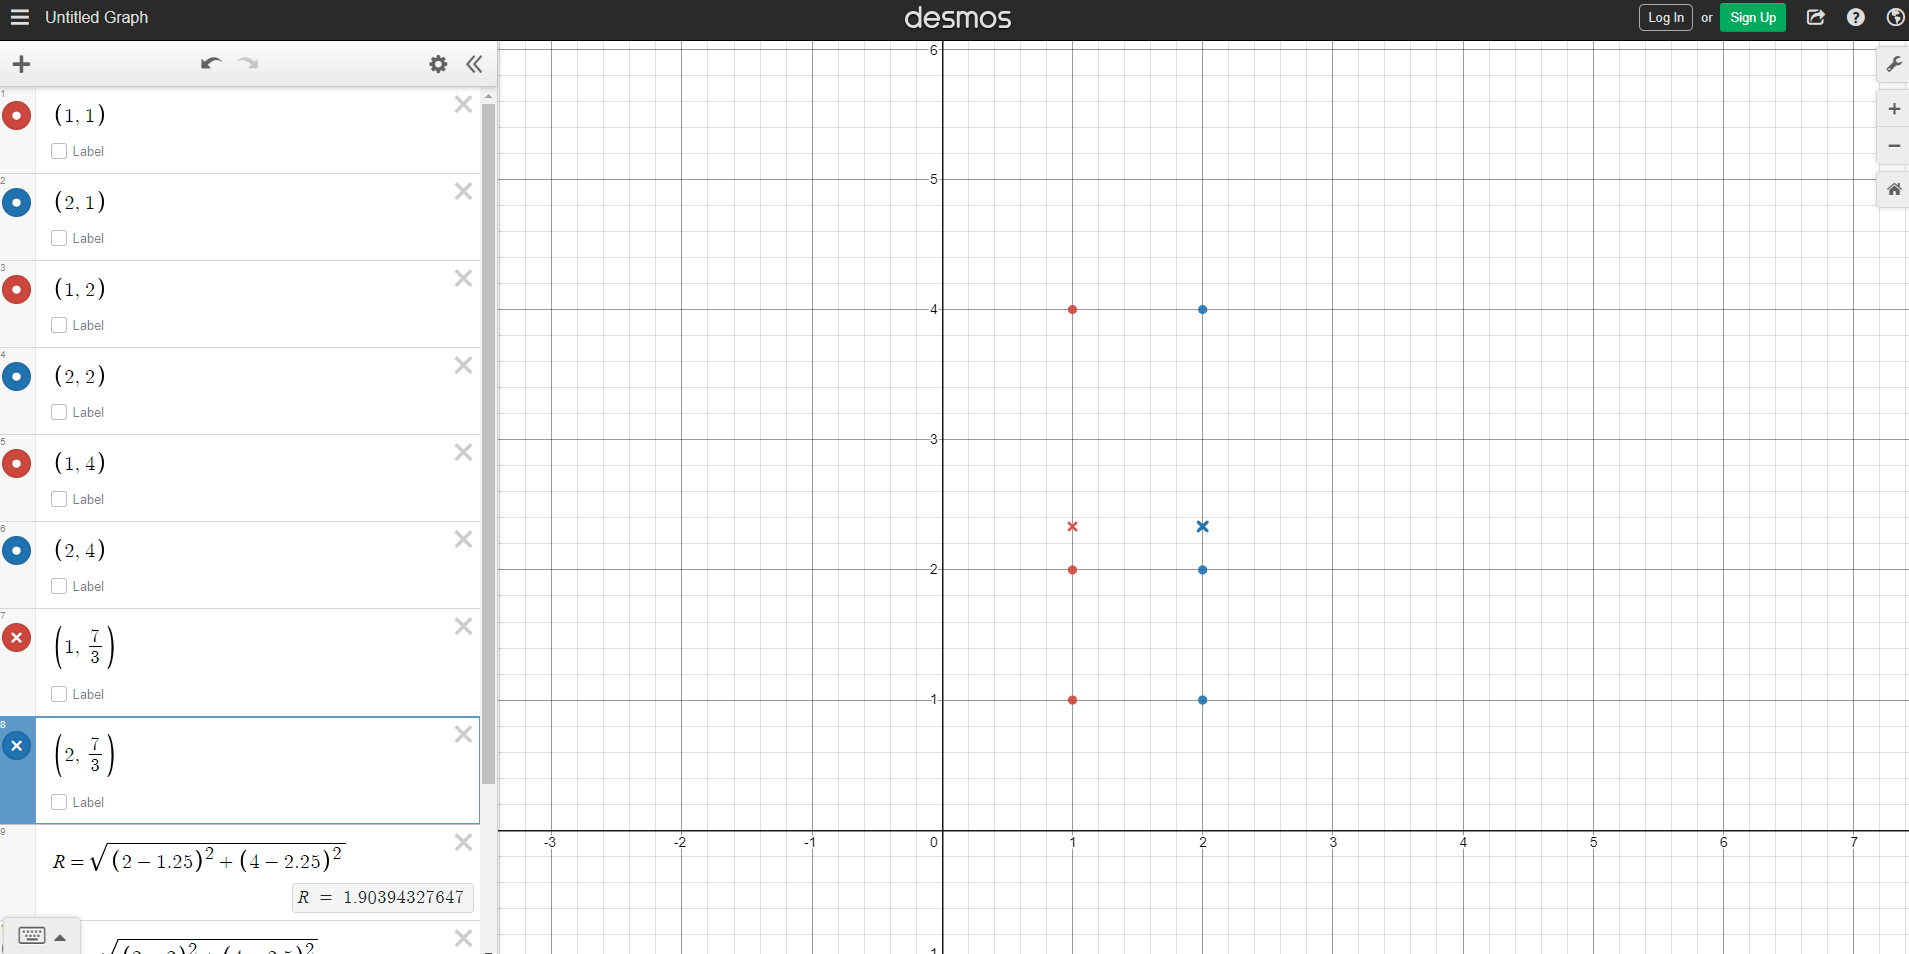
\includegraphics[scale = .3]{2c.png}
        \item These do not look like the two centroids which minimize the variation within
        each cluster. If we had the two centroids between the top two points and in the 
        middle of the bottom four points, that would minimize the variation within each cluster. 
    \end{enumerate}

    \item If we assign $C_1$ with observations 1, 3, and 5 and $C_2$ with the observations 
    2, 4, and 6 we reach the convergece of the previous example, where we said these centroids 
    do not minimize the variations in the groups. 
\end{enumerate}

\end{document}